\let\negmedspace\undefined
\let\negthickspace\undefined
\documentclass[journal]{IEEEtran}
\usepackage[a5paper, margin=10mm, onecolumn]{geometry}
%\usepackage{lmodern} % Ensure lmodern is loaded for pdflatex
\usepackage{tfrupee} % Include tfrupee package

\setlength{\headheight}{1cm} % Set the height of the header box
\setlength{\headsep}{0mm}     % Set the distance between the header box and the top of the text

\usepackage{gvv-book}
\usepackage{gvv}
\usepackage{cite}
\usepackage{amsmath,amssymb,amsfonts,amsthm}
\usepackage{algorithmic}
\usepackage{graphicx}
\usepackage{textcomp}
\usepackage{xcolor}
\usepackage{txfonts}
\usepackage{listings}
\usepackage{enumitem}
\usepackage{mathtools}
\usepackage{gensymb}
\usepackage{comment}
\usepackage[breaklinks=true]{hyperref}
\usepackage{tkz-euclide} 
\usepackage{listings}
% \usepackage{gvv}                                        
\def\inputGnumericTable{}                                 
\usepackage[latin1]{inputenc}                                
\usepackage{color}                                            
\usepackage{array}                                            
\usepackage{longtable}                                       
\usepackage{calc}                                             
\usepackage{multirow}                                         
\usepackage{hhline}                                           
\usepackage{ifthen}                                           
\usepackage{lscape}
\usepackage{circuitikz}


\renewcommand{\thefigure}{\theenumi}
\renewcommand{\thetable}{\theenumi}
\setlength{\intextsep}{10pt} % Space between text and floats


\numberwithin{equation}{enumi}
\numberwithin{figure}{enumi}
\renewcommand{\thetable}{\theenumi}


% Marks the beginning of the document
\begin{document}
\bibliographystyle{IEEEtran}
\vspace{3cm}

\title{GATE 2022}
\author{EE25BTECH11065 - YOSHITA.J}
\maketitle

% (add your content here)
\noindent \textbf{Q. 1 -- Q. \textbf{5}} carry one mark each.

\begin{enumerate}
    \item You should \rule{3cm}{0.15mm} when to say \rule{3cm}{0.15mm}
    \begin{enumerate}
        \item  no / no
        \item  no / know
        \item  know / know
        \item  know / no
    \end{enumerate}
    \hfill{$\brak{ GATE\ EY\ 2022}$}
    \bigskip
     \item Two straight lines pass through the origin $(x_0, y_0) = (0,0)$. One of them passes
through the point $(x_1, y_1) = (1,3)$ and the other passes through the point
$(x_2,y_2) = (1,2)$.
\\
What is the area enclosed between the straight lines in the interval $\sbrak{0, 1}$ on
the $x$-axis?
    \begin{enumerate}
        \item  $0.5$
        \item  $1.0$
        \item  $1.5$
        \item  $2.0$
    \end{enumerate}
    \hfill{$\brak{ GATE\ EY\ 2022}$}
    \bigskip
     \item If

$p:q=1:2$

$q:r = 4:3$

$r : s = 4:5$

and u is $50\%$ more than s, what is the ratio $p : u$?
    \begin{enumerate}
        \item  $2:15$
        \item  $16:15$
        \item  $1:5$
        \item  $16:45$
    \end{enumerate}
    \hfill{$\brak{ GATE\ EY\ 2022}$}
    \bigskip
     \item Given the statements:
     \begin{itemize}[label=$\bullet$]
    \item P is the sister of Q.
    \item Q is the husband of R.
    \item R is the mother of S.
    \item T is the husband of P.
   \end{itemize}
    
Based on the above information, T is \rule{3cm}{0.15mm} of S.
    \begin{enumerate}
        \item  the grandfather
        \item  an uncle
        \item  the father
        \item  a brother
    \end{enumerate}
    \hfill{$\brak{ GATE\ EY\ 2022}$}
    \bigskip
     \item In the following diagram, the point R is the center of the circle. The lines PQ
and ZV are tangential to the circle. The relation among the areas of the squares,
PXWR, RUVZ and SPQT is
\begin{figure}[H]
    \centering
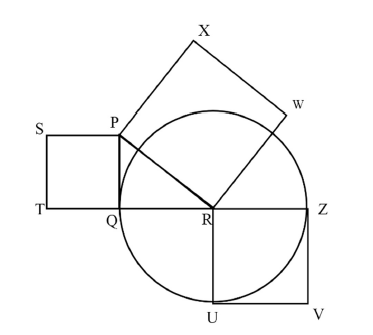
\includegraphics[width=0.5\columnwidth]{figs/1.png}
    \caption{}
    \label{fig:1}
   \end{figure}
    \begin{enumerate}
        \item  Area of SPQT = Area of RUVZ = Area of PXWR
        \item  Area of SPQT = Area of PXWR - Area of RUVZ
        \item  Area of PXWR = Area of SPQT - Area of RUVZ
        \item  Area of PXWR = Area of RUVZ - Area of SPQT
    \end{enumerate}
    \hfill{$\brak{ GATE\ EY\ 2022}$}
    \bigskip
         \item 
         Healthy eating is a critical component of healthy aging. When should one start
eating healthy? It turns out that it is never too early. For example, babies who
start eating healthy in the first year are more likely to have better overall health
as they get older.

Which one of the following is the CORRECT logical inference based on the
information in the above passage?
    \begin{enumerate}
        \item  Healthy eating is important for those with good health conditions, but not for
others
        \item  Eating healthy can be started at any age, earlier the better
        \item  Eating healthy and better overall health are more correlated at a young age, but
not older age
        \item  Healthy eating is more important for adults than kids
    \end{enumerate}
    \hfill{$\brak{ GATE\ EY\ 2022}$}
    \bigskip
    
     \item P invested \rupee5000 per month for $6$ months of a year and Q invested \rupee $x$  per
month for $8$ months of the year in a partnership business. The profit is shared in
proportion to the total investment made in that year.
If at the end of that investment year, Q receives $\frac{4}{9}$ 
of the total profit, what is the
value of $x$ (in \rupee)?
    \begin{enumerate}
        \item  $2500$
        \item  $3000$
        \item  $4687$
        \item  $4687$
    \end{enumerate}
    \hfill{$\brak{ GATE\ EY\ 2022}$}
    \bigskip
 \item  .
 \begin{figure}[H]
    \centering
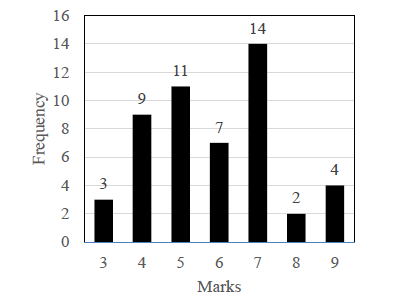
\includegraphics[width=0.5\columnwidth]{figs/2.png}
    \caption{}
    \label{fig:2}
   \end{figure}
   
   The above frequency chart shows the frequency distribution of marks obtained
by a set of students in an exam.
From the data presented above, which one of the following is CORRECT?
    \begin{enumerate}
        \item  mean $>$ mode $>$ median
        \item  mode $>$ median $>$ mean
        \item  mode $>$ mean $>$ median
        \item  median $>$ mode $>$ mean
    \end{enumerate}
    \hfill{$\brak{ GATE\ EY\ 2022}$}
    \bigskip
 \item In the square grid shown on the left, a person standing at P$2$ position is required
to move to P$5$ position.
The only movement allowed for a step involves, ``two moves along one direction followed by one move in a perpendicular direction`` The permissible directions for movement are shown as dotted arrows in the right.
For example, a person at a given position Y can move only to the positions
marked X on the right.
Without occupying any of the shaded squares at the end of each step, the
minimum number of steps required to go from P$2$ to P$5$ is
\begin{figure}[H]
    \centering
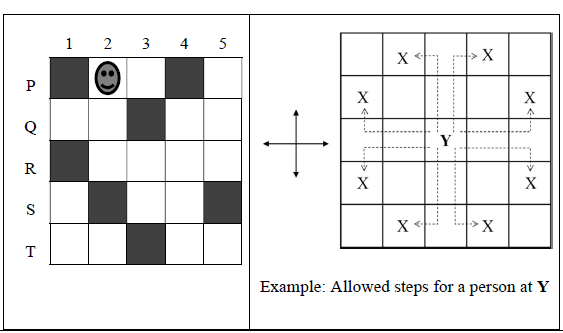
\includegraphics[width=0.5\columnwidth]{figs/3.png}
    \caption{}
    \label{fig:3}
   \end{figure}
    \begin{enumerate}
        \item  $4$
        \item  $5$
        \item  $6$
        \item  $7$
    \end{enumerate}
    \hfill{$\brak{ GATE\ EY\ 2022}$}
    \bigskip
 \item .
 \begin{figure}[H]
    \centering
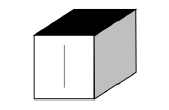
\includegraphics[width=0.5\columnwidth]{figs/4.png}
    \caption{}
    \label{fig:4}
   \end{figure}
 Consider a cube made by folding a single sheet of paper of appropriate shape.
The interior faces of the cube are all blank. However, the exterior faces that are
not visible in the above view may not be blank.
Which one of the following represents a possible unfolding of the cube?
\begin{figure}[H]
    \centering
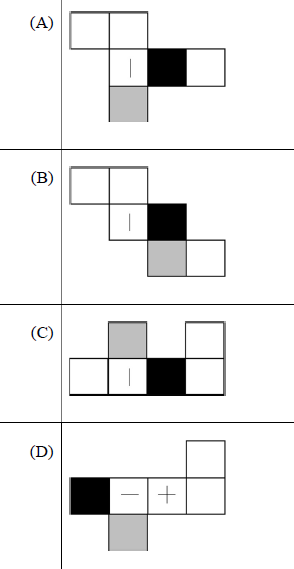
\includegraphics[width=0.5\columnwidth]{figs/5.png}
    \caption{}
    \label{fig:5}
   \end{figure}
    \hfill{$\brak{ GATE\ EY\ 2022}$}
    \bigskip
    \noindent \textbf{Q. 11 -- Q. \textbf{35}} carry one mark each.
  \item Which one of the following options denotes the time when the majority of animal
phyla first appeared in the fossil record? $\brak{MYA\ =\ Million\ Years\ Ago}$
    \begin{enumerate}
        \item  $65 MYA$
        \item  $250 MYA$
        \item  $550 MYA$
        \item  $700 MYA$
    \end{enumerate}
    \hfill{$\brak{ GATE\ EY\ 2022}$}
    \bigskip
 \item Consider the following strains of an influenza virus and their basic reproduction
numbers $\brak{R_0}$. Assuming that they are all equally virulent, which one of the
following strains would be most concerning for a completely vulnerable
population of humans?
    \begin{enumerate}
        \item  $\alpha$-strain with $R_0$ = $4.0$
        \item  $\beta$-strain with $R_0$ = $1.0$
        \item  $\gamma$-strain with $R_0$ = $0.5$
        \item  $\delta$-strain with $R_0$ = $0.2$
    \end{enumerate}
    \hfill{$\brak{ GATE\ EY\ 2022}$}
    \bigskip
 \item Which one of the following statements is true with respect to energy requirements
of photosynthesis in $C3$ and $C4$ biochemical cycles?
    \begin{enumerate}
        \item  $C3 > C4$
        \item  $C4 > C3$
        \item  $C3 = C4$
        \item  Energy requirement is unrelated to $C3$ or $C4$cycle
    \end{enumerate}
    \hfill{$\brak{ GATE\ EY\ 2022}$}
    \bigskip
 \item Which one of the following is a proximate explanation for grouping in animals?
    \begin{enumerate}
        \item  Animals in groups face a lower risk of predation.
        \item  Animals form groups to forage efficiently
        \item  Groups can navigate their environment better
        \item  Groups form when individuals show attraction to others
    \end{enumerate}
    \hfill{$\brak{ GATE\ EY\ 2022}$}
    \bigskip
 \item The ethologist Konrad Lorenz is known for his discovery of which one of the
following processes?
    \begin{enumerate}
        \item  Habituation
        \item  Sensitization
        \item  Reinforcement
        \item  Imprinting
    \end{enumerate}
    \hfill{$\brak{ GATE\ EY\ 2022}$}
    \bigskip
 \item Male stickleback fish develop red colour on their ventral side in the breeding
season and maintain territories. When a conspecific male intruder enters their
territory, resident males perform an aggressive display. The ethologist Niko
Tinbergen presented models of different shapes to territorial male stickleback fish.
He found that models of any shape elicited aggressive displays, provided the
ventral part of the models was coloured red. This observation led to the
development of which one of the following concepts
    \begin{enumerate}
        \item  Supernormal stimuli
        \item  Sign stimuli
        \item  Gestalt stimuli
        \item  Internal stimuli
    \end{enumerate}
    \hfill{$\brak{ GATE\ EY\ 2022}$}
    \bigskip
 \item Neuronal circuits that mediate escape responses in animals would perform best if
they had which one of the following combination of properties?
    \begin{enumerate}
        \item  Large diameter axons and electrical synapses
        \item  Small diameter axons and electrical synapses
        \item  Large diameter axons and chemical synapses
        \item  Small diameter axons and chemical synapses
    \end{enumerate}
    \hfill{$\brak{ GATE\ EY\ 2022}$}
    \bigskip
 \item Moth caterpillars that mimic bird droppings are an example of which one of the
following phenomena?
    \begin{enumerate}
        \item  Aposematism
        \item  Batesian mimicry
        \item  Masquerade
        \item  Müllerian mimicry
    \end{enumerate}
    \hfill{$\brak{ GATE\ EY\ 2022}$}
    \bigskip
 \item Which one of the following processes is not likely to lead to the stable
coexistence of two species at the same trophic level within an ecological
community?
    \begin{enumerate}
        \item  Density-dependent predation
        \item  Facilitation
        \item  Intense interspecific competition
        \item  Niche differentiation
    \end{enumerate}
    \hfill{$\brak{ GATE\ EY\ 2022}$}
    \bigskip
 \item Which one of the following organisms is a cytoplasmically inherited symbiotic
bacterium that can cause extreme female-biased sex ratios in many insects?
    \begin{enumerate}
        \item  $Clostridium$
        \item  $Escherichia$
        \item  $Mycobacterium$
        \item  $Wolbachia$
    \end{enumerate}
    \hfill{$\brak{ GATE\ EY\ 2022}$}
    \bigskip
 \item A cross between a pure-bred plant with red flowers and a pure-bred plant with
white flowers produced F1 generation with pink flowers. If the plants with pink
flowers are selfed, what is the proportion of white : pink : red flowers expected in
the next generation?
    \begin{enumerate}
        \item  $1 : 1 : 1$
        \item  $1 : 2 : 1$
        \item  $2 : 1 : 2$
        \item  $2 : 2 : 1$
    \end{enumerate}
    \hfill{$\brak{ GATE\ EY\ 2022}$}
    \bigskip
 \item A gene coding for a particular protein exhibits 2\% DNA sequence divergence
between humans and chimpanzees. However, protein sequences encoded by them
are identical. Which one of the following processes explains this?
    \begin{enumerate}
        \item  Nonsynonymous changes in the gene sequences
        \item  Synonymous changes in the gene sequences
        \item  Nonsense mutations in the gene sequences
        \item  Frameshift mutations in the gene sequences
    \end{enumerate}
    \hfill{$\brak{ GATE\ EY\ 2022}$}
    \bigskip
 \item Which one of the following sets of characteristics is most likely to cause
population extinction via demographic stochasticity?
    \begin{enumerate}
        \item  Small geographical range and low population density
        \item  Large geographical range and low population density
        \item  Small geographical range and high population density
        \item  Large geographical range and high population density
    \end{enumerate}
    \hfill{$\brak{ GATE\ EY\ 2022}$}
    \bigskip
 \item Which one of the following is not an expected impact of global warming?
    \begin{enumerate}
        \item  Birds shifting their distributions to higher elevations
        \item  Fish shifting their distributions to deeper waters
        \item  Lizards shifting their distributions towards the equator
        \item  Mammals shifting their distributions towards higher latitudes
    \end{enumerate}
    \hfill{$\brak{ GATE\ EY\ 2022}$}
    \bigskip
 \item Which one of the following represents the chemical energy available to herbivores
in an ecosystem?
    \begin{enumerate}
        \item  Net Secondary Productivity
        \item  Gross Primary Productivity
        \item  Net Ecosystem Productivity
        \item  Net Primary Productivity
    \end{enumerate}
    \hfill{$\brak{ GATE\ EY\ 2022}$}
    \bigskip
 \item Which one of the following major mass extinctions is the most recent?
    \begin{enumerate}
        \item  Cretaceous-Paleogene
        \item  Late Devonian
        \item  Permian-Triassic
        \item  Triassic-Jurassic
    \end{enumerate}
    \hfill{$\brak{ GATE\ EY\ 2022}$}
    \bigskip
 \item Which one of the following does not help maintain genetic diversity at a given
locus?
    \begin{enumerate}
        \item  Heterozygote advantage
        \item  Genetic drift
        \item  Negative frequency dependent selection
        \item  Mutation-Selection balance
    \end{enumerate}
    \hfill{$\brak{ GATE\ EY\ 2022}$}
    \bigskip
 \item Which one of the following is potentially explained by the mid-domain effect?
    \begin{enumerate}
        \item  Increase in body size of mammals at high latitudes
        \item  Species richness along an elevational gradient
        \item  Cumulative species richness with increasing area
        \item  Species richness along a disturbance gradient
    \end{enumerate}
    \hfill{$\brak{ GATE\ EY\ 2022}$}
    \bigskip
 \item The graph shows the yield of coffee plantations located at different distances from
a patch of primary forest
\begin{figure}[H]
    \centering
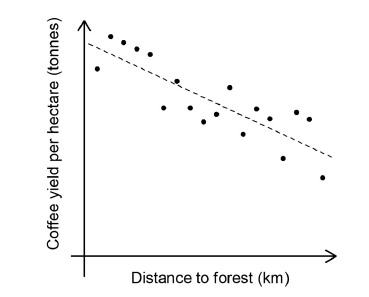
\includegraphics[width=0.5\columnwidth]{figs/6.png}
    \caption{}
    \label{fig:6}
   \end{figure}
Which one of the following options best explains this pattern?
    \begin{enumerate}
        \item  Carbon sequestration
        \item  Seed predation by forest-dwelling insects
        \item  Pollination by forest-dwelling insects
        \item  Seed dispersal by forest-dwelling birds and mammals
    \end{enumerate}
    \hfill{$\brak{ GATE\ EY\ 2022}$}
    \bigskip
 \item Which one or more of the following bird species is/are the focus of
conservation-oriented captive breeding efforts in India?
    \begin{enumerate}
        \item  Great Indian Bustard
        \item  Himalayan Quail
        \item  Jerdon's Courser
        \item  White-winged Wood Duck
    \end{enumerate}
    \hfill{$\brak{ GATE\ EY\ 2022}$}
    \bigskip
 \item Which one or more of the following is/are not an example of a zoonotic
disease$\brak{s}$?
    \begin{enumerate}
        \item  Ebola
        \item  HIV-AIDS
        \item  Lyme disease
        \item  Poliomyelitis
    \end{enumerate}
    \hfill{$\brak{ GATE\ EY\ 2022}$}
    \bigskip
 \item   Small islands tend to have fewer species than nearby large islands. Which one or
more of the following reasons explain(s) this outcome?
    \begin{enumerate}
        \item  Smaller areas have higher extinction rates.
        \item  Smaller areas have low environmental heterogeneity.
        \item  Smaller areas support smaller populations.
        \item  Smaller areas have higher speciation rates.
    \end{enumerate}
    \hfill{$\brak{ GATE\ EY\ 2022}$}
    \bigskip
 \item The term ``living fossil`` applies to which one or more of the following organisms?
    \begin{enumerate}
        \item  Coelacanth
        \item  Echidna
        \item  Horseshoe crab
        \item  Rhinoceros viper
    \end{enumerate}
    \hfill{$\brak{ GATE\ EY\ 2022}$}
    \bigskip
 \item Which one or more of the following reasons has/have been invoked to explain
island gigantism?
    \begin{enumerate}
        \item  Absence of interspecific competitors
        \item  Absence of predators
        \item  Limited habitat
        \item  Limited prey base
    \end{enumerate}
    \hfill{$\brak{ GATE\ EY\ 2022}$}
    \bigskip
 \item Which one or more of the following options represent(s) life history trade-offs?
    \begin{enumerate}
        \item  Egg size versus clutch size
        \item  Growth versus age at sexual maturation
        \item  Mate choice versus offspring quality
        \item  Survival versus reproduction
    \end{enumerate}
    \hfill{$\brak{ GATE\ EY\ 2022}$}
    \bigskip
 \item Certain plants and animals rely on toxins such as cardiac glycosides for self-defense.
Digitoxin and bufalin, structurally similar toxins produced by foxglove plants and
bufonid toads, respectively, are one such example. Which one of the following
statements about these toxins is correct?
    \begin{enumerate}
        \item  They are structural and functional analogs.
        \item  They are structural and functional homologs.
        \item  They are structural analogs and functional homologs.
        \item  They are structural homologs and functional analogs
    \end{enumerate}
    \hfill{$\brak{ GATE\ EY\ 2022}$}
    \bigskip
 \item A behavioural ecologist records the number of times a kingfisher succeeds in catching
fish over multiple five-minute intervals. Which one of the following distributions best
describes these data?
    \begin{enumerate}
        \item  Chi-squared
        \item  Normal
        \item  Poisson
        \item  Student's-t
    \end{enumerate}
    \hfill{$\brak{ GATE\ EY\ 2022}$}
    \bigskip
 \item Excess fertilizers used in agriculture commonly end up as runoff and cause
phytoplankton blooms in rivers. To figure out whether these blooms were driven by
ammonium or phosphate fertilizers, researchers cultured a phytoplankton species in
multiple samples of unpolluted river water. The samples were divided equally among
three treatments: ammonium fertilizer added, phosphate fertilizer added and no
fertilizer added. They then measured phytoplankton density in each of the samples
after a week. Phytoplankton densities (in thousands of cells/ml) are reported in the
table shown.
\begin{figure}[H]
    \centering
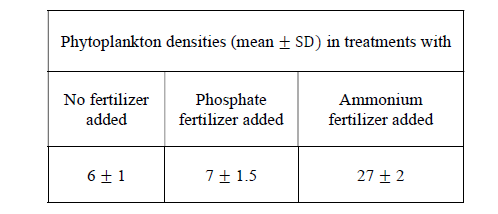
\includegraphics[width=0.5\columnwidth]{figs/7.png}
    \caption{}
    \label{fig:7}
   \end{figure}
Which one of the following inferences is correct?
    \begin{enumerate}
        \item  Nitrogen is the limiting nutrient for phytoplankton growth
        \item  Phosphorus is the limiting nutrient for phytoplankton growth.
        \item  Both nitrogen and phosphorus limit phytoplankton growth.
        \item  Neither nitrogen nor phosphorus limits phytoplankton growth
    \end{enumerate}
    \hfill{$\brak{ GATE\ EY\ 2022}$}
    \bigskip
 \item $S1$ and $S2$ are two strains of bacteria. The results of a bacterial growth experiment
on these strains measured after $24$ hours are shown. Black and white bars represent
$S1$ and $S2$, respectively.
\begin{figure}[H]
    \centering
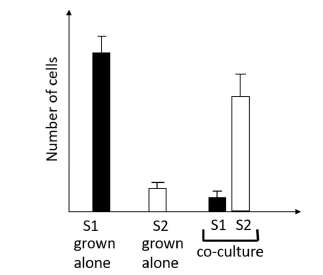
\includegraphics[width=0.5\columnwidth]{figs/8.png}
    \caption{}
    \label{fig:8}
   \end{figure}
Which one of the following best describes the interaction between $S1$ and $S2$?
    \begin{enumerate}
        \item  Amensalism
        \item  Commensalism
        \item  Cooperator-cheater
        \item  Mutualism
    \end{enumerate}
    \hfill{$\brak{ GATE\ EY\ 2022}$}
    \bigskip
 \item Habitat P has twice the density of resources as habitat Q. Assume that individuals are
identical, can move freely, have perfect information about the environment, and
compete for resources when they are in a habitat. At equilibrium, which one of the
following represents the predicted outcome?
    \begin{enumerate}
        \item  The number of individuals present and the profitability per individual will be higher in
P than in Q.
        \item  The number of individuals present and the profitability per individual will be the same
in P and in Q.
        \item  The number of individuals present will be higher in P than in Q and the profitability
per individual will be the same in P and in Q.
        \item  The number of individuals present will be higher in Q than in P and the profitability
per individual will be higher in P than in Q.
    \end{enumerate}
    \hfill{$\brak{ GATE\ EY\ 2022}$}
    \bigskip
 \item Consider Holling's Type-III functional response, as shown.
 \begin{figure}[H]
    \centering
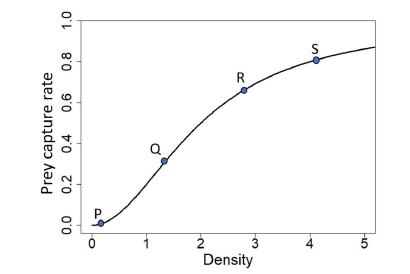
\includegraphics[width=0.5\columnwidth]{figs/9.png}
    \caption{}
    \label{fig:9}
   \end{figure}
 Which one of the marked points has the highest rate-of-change of prey-capture-rate?
    \begin{enumerate}
        \item  P
        \item  Q
        \item  R
        \item  S
    \end{enumerate}
    \hfill{$\brak{ GATE\ EY\ 2022}$}
    \bigskip
 \item In a population of birds on an island, the average beak size reduced over one
generation. A researcher estimated the association between beak size and relative fitness, shown in the graph. the estimated slope was-$0.05$ with a $95$\% confidence interval of -$0.15$ to $0.09$.

\begin{figure}[H]
    \centering
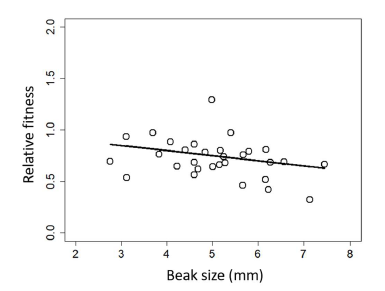
\includegraphics[width=0.5\columnwidth]{figs/10.png}
    \caption{}
    \label{fig:10}
   \end{figure}
Which one of the following evolutionary processes acting on beak size is the most
likely reason for the observed reduction in beak size?
    \begin{enumerate}
        \item  Genetic drift
        \item  Group selection
        \item  Kin selection
        \item  Natural selection
    \end{enumerate}
    \hfill{$\brak{ GATE\ EY\ 2022}$}
    \bigskip
  \item The Bateman gradient is a popular explanation for why the strength of sexual selection
is typically stronger on males than on females. Which one of the following figures is
the correct representation of the Bateman gradient? In all figures, the dotted line
represents males and the solid line females
\begin{figure}[H]
    \centering
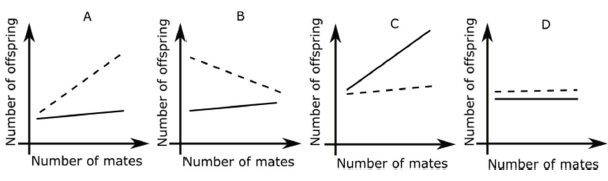
\includegraphics[width=0.5\columnwidth]{figs/11.png}
    \caption{}
    \label{fig:11}
   \end{figure}
    \begin{enumerate}
        \item  A
        \item  B
        \item  C
        \item  D
    \end{enumerate}
    \hfill{$\brak{ GATE\ EY\ 2022}$}
    \bigskip
 \item Sparrows use two foraging tactics to obtain food. They either search for grains
themselves $\brak{Producer\ tactic\ P}$ or follow other individuals and steal grains from them
$\brak{Scrounger\ tactic\ S}$. The following graphs show how the fitness of each tactic
$\brak{P\ :\ dashed\ line\ and\ S\ :\ solid\ line}$ varies as a function of the relative frequency of S.
Which one of the graphs shows the correct representation of these tactics if they were
maintained through negative frequency dependence?
\begin{figure}[H]
    \centering
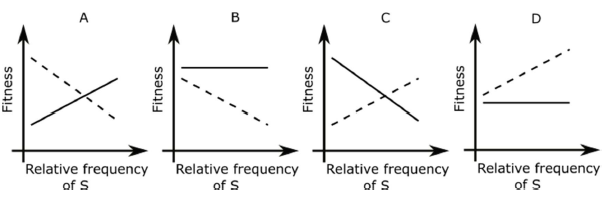
\includegraphics[width=0.5\columnwidth]{figs/12.png}
    \caption{}
    \label{fig:12}
   \end{figure}
    \begin{enumerate}
        \item  A
        \item  B
        \item  C
        \item  D
    \end{enumerate}
    \hfill{$\brak{ GATE\ EY\ 2022}$}
    \bigskip
 \item Some lizard species show positive allometry in head width, with larger individuals
investing disproportionately more in musculature leading to wider heads. To test for
positive allometry in a study population, a researcher measures body size and head
width for $100$ individuals and fits a straight line to a log-log plot of these two traits.
Which one of the following estimated values of the slope indicates support for
positive allometry?
    \begin{enumerate}
        \item  $0$
        \item  $0.5$
        \item  $1$
        \item  $1.5$
    \end{enumerate}
    \hfill{$\brak{ GATE\ EY\ 2022}$}
    \bigskip
 \item A team of ecologists laid $100$ plots of $50\,\text{m} \times 50\,\text{m}$ in a forest and counted the number
of individuals of a tree species in each plot. They then calculated the mean and
variance of the number of individuals per plot. If trees are randomly distributed, then
which one of the following relationships between the variance and mean is expected?
    \begin{enumerate}
        \item  Variance $>$ mean
        \item  Variance $<$ mean
        \item  Variance = mean
        \item  Variance is independent of the mean
    \end{enumerate}
    \hfill{$\brak{ GATE\ EY\ 2022}$}
    \bigskip
 \item The following graphs show rank abundance data for species in three different
communities P, Q and R. Based on both species richness and relative abundance,
which one of the following options correctly represents the ordering of communities
according to their species diversity?
\begin{figure}[H]
    \centering
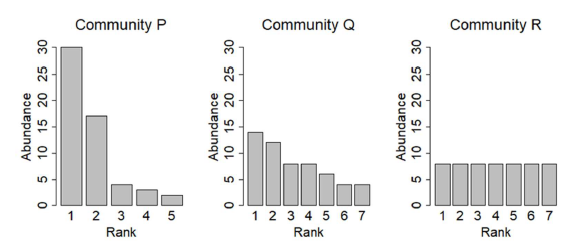
\includegraphics[width=0.5\columnwidth]{figs/13.png}
    \caption{}
    \label{fig:13}
   \end{figure}
    \begin{enumerate}
        \item  $P > Q > R$
        \item  $Q > P > R$
        \item  $R > P > Q$
        \item  $R > Q > P$
    \end{enumerate}
    \hfill{$\brak{ GATE\ EY\ 2022}$}
    \bigskip
 \item Which one of the following cladograms represents the correct phylogenetic
relationships in the Kingdom Animalia?
\begin{figure}[H]
    \centering
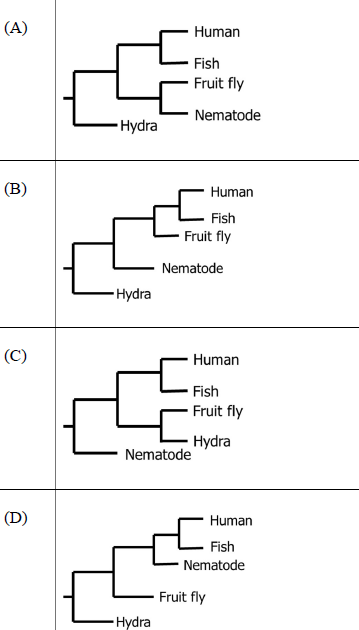
\includegraphics[width=0.5\columnwidth]{figs/14.png}
    \caption{}
    \label{fig:14}
   \end{figure}
    \hfill{$\brak{ GATE\ EY\ 2022}$}
    \bigskip
 \item $\beta$-diversity quantifies the difference in species composition between two ecological
communities. Which one of the following statements is correct about $\beta$-diversity?
    \begin{enumerate}
        \item  Only nestedness affects $\beta$-diversity.
        \item  Only species turnover affects $\beta$-diversity.
        \item  Both nestedness and species turnover affect $\beta$-diversity
        \item  Neither nestedness nor species turnover affects $\beta$-diversity
    \end{enumerate}
    \hfill{$\brak{ GATE\ EY\ 2022}$}
    \bigskip
 \item Consider the logistic population growth model, given by
\[
\frac{dn}{dt} = r n \left( 1 - \frac{n}{k} \right)
\]

 where r is the intrinsic growth rate, n is the population size and k is the carrying
capacity. Which one or more of the following is/are assumption$\brak{s}$ of the model?
    \begin{enumerate}
        \item  Carrying capacity is constant
        \item  Density dependence is quadratic
        \item  Continuous growth with no time-lags
        \item  No genetic, age or size structure
    \end{enumerate}
    \hfill{$\brak{ GATE\ EY\ 2022}$}
    \bigskip
 \item Which one or more of the following genes/markers is/are typically used for species
identification?
    \begin{enumerate}
        \item  $16S$ rRNA
        \item  Cytochrome Oxidase I
        \item  IgG
        \item  Microsatellites
    \end{enumerate}
    \hfill{$\brak{ GATE\ EY\ 2022}$}
    \bigskip
 \item A bee species forages for nectar on a plant species which has yellow flowers. To find
out what cues the bees use to recognize the flowers, researchers performed the
following experiment. They presented individual bees with the stimuli given below
and examined the proportion of bees that approached and landed on the stimuli.
The results are shown below.
\begin{figure}[H]
    \centering
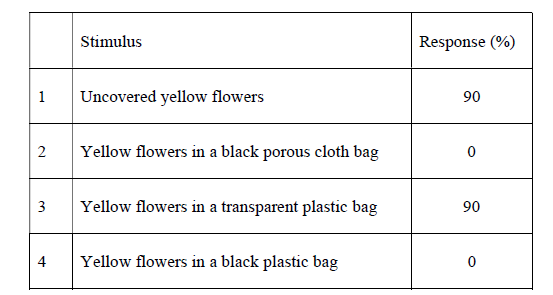
\includegraphics[width=0.5\columnwidth]{figs/15.png}
    \caption{}
    \label{fig:15}
   \end{figure}
Which one or more of the following interpretation$\brak{s}$ of the experiment is/are correct?
    \begin{enumerate}
        \item  All flower colours other than yellow are ineffective at eliciting approach responses
        \item  Olfactory cues are sufficient to elicit approach responses.
        \item  Visual cues are necessary to elicit approach responses.
        \item  Visual cues are sufficient to elicit approach responses.
    \end{enumerate}
    \hfill{$\brak{ GATE\ EY\ 2022}$}
    \bigskip
 \item Which one or more of the following reason$\brak{s}$ explain$\brak{s}$ why whales use low
frequencies $\brak{infrasound}$ for mate-finding and high frequencies $\brak{ultrasound}$
for hunting prey?
    \begin{enumerate}
        \item  High frequencies transmit further without distortion than low frequencies.
        \item  High frequencies scatter more and allow for high-resolution information
        \item  Low frequencies transmit further without distortion than high frequencies.
        \item  Low frequencies scatter more and allow for high-resolution information
    \end{enumerate}
    \hfill{$\brak{ GATE\ EY\ 2022}$}
    \bigskip
 \item The table shows the relative abundance of three potential prey species in the
environment and in the diet of a bat predator.
\begin{figure}[H]
    \centering
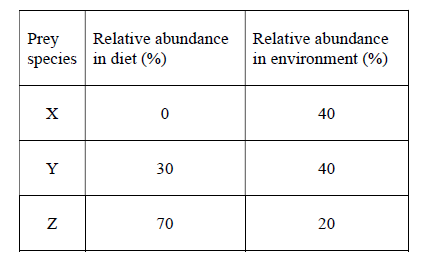
\includegraphics[width=0.5\columnwidth]{figs/16.png}
    \caption{}
    \label{fig:16}
   \end{figure}
Which one or more of the following is/are possible interpretations based on the data?
    \begin{enumerate}
        \item  The predator shows a preference for prey species Z.
        \item  The predator shows no preference for any of the three prey species.
        \item  Species X is avoided by the predator.
        \item  The predator shows a preference for prey species Y.
    \end{enumerate}
    \hfill{$\brak{ GATE\ EY\ 2022}$}
    \bigskip
 \item Which one or more of the following options represent$\brak{s}$ an evolutionary arms race?
    \begin{enumerate}
        \item Snake venom toxin specificity and prey receptor modification 
        \item  Egg discrimination by hosts and brood parasite egg colouration
        \item  Cooperative breeding and offspring survival rate
        \item  Crypsis in prey and visual acuity in predator
    \end{enumerate}
    \hfill{$\brak{ GATE\ EY\ 2022}$}
    \bigskip
 \item The figure shows an $F$ probability density function. The two dotted lines represent
critical values corresponding to a two-tailed $F$-test at a level of significance of $0.05$.
The observed $F$-statistic for two samples is indicated by the solid line.
\begin{figure}[H]
    \centering
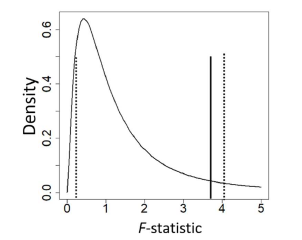
\includegraphics[width=0.5\columnwidth]{figs/17.png}
    \caption{}
    \label{fig:17}
   \end{figure}
Which one or more of the following inferences is/are correct?
    \begin{enumerate}
        \item  The null hypothesis cannot be rejected
        \item  The null hypothesis is true.
        \item  The ratio of the variances of the two samples is not statistically significantly
different from $1$.
        \item  The ratio of the skewness of the two samples is not statistically significantly
different from $1$
    \end{enumerate}
    \hfill{$\brak{ GATE\ EY\ 2022}$}
    \bigskip
 \item Which one or more of the following conditions can lead to an increase in tree densities
in tropical savannas?
    \begin{enumerate}
        \item  Fire suppression
        \item  Increase in mean annual rainfall
        \item  Increased levels of browsing by herbivores
        \item  Increased atmospheric $CO_2$
    \end{enumerate}
    \hfill{$\brak{ GATE\ EY\ 2022}$}
    \bigskip
 \item Gene conversion can lead to which one or more of the following evolutionary
outcomes?
    \begin{enumerate}
        \item  Concerted evolution
        \item  Increased expression
        \item  Increased sequence divergence
        \item  Increased sequence similarity
    \end{enumerate}
    \hfill{$\brak{ GATE\ EY\ 2022}$}
    \bigskip
 \item If the observed heterozygosity at a locus is $0.6$, which one or more of the following
could produce this outcome?
    \begin{enumerate}
        \item  A neutral locus with three alleles
        \item  A locus under selection with two alleles
        \item  A neutral locus with two alleles
        \item  A locus under selection with one allele
    \end{enumerate}
    \hfill{$\brak{ GATE\ EY\ 2022}$}
    \bigskip
 \item Which one or more of the following reasons has/have been invoked to explain high
species diversity in the tropics?
    \begin{enumerate}
        \item  Greater area in the tropics
        \item  Higher speciation rates in the tropics
        \item  Lower extinction rates in the tropics
        \item  The tropics are closer to the sun
    \end{enumerate}
    \hfill{$\brak{ GATE\ EY\ 2022}$}
    \bigskip
 \item In a linear regression with a single continuous predictor and $100$ data points, the
residual degrees of freedom are \rule{3cm}{0.15mm} . $\brak{Answer\ in\ integer}$
    \hfill{$\brak{ GATE\ EY\ 2022}$}
    \bigskip
 \item The genome of an organism has $60$\% GC $\brak{Guanine-Cytosine}$ content.
The Adenine in this genome is \rule{3cm}{0.15mm} \% . $\brak{Answer\ in\ integer}$
    \hfill{$\brak{ GATE\ EY\ 2022}$}
    \bigskip
\item The prevalence of flu in a population is $1$\%. A diagnostic test has a false positive rate
of 10 and a false negative rate of $10$\%. The probability that a randomly chosen
person tests positive is \rule{3cm}{0.15mm} . $\brak{Round\ off\ to\ three\ decimal\ places}$
    \hfill{$\brak{ GATE\ EY\ 2022}$}
    \bigskip
 \item In a deer population, the male-to-female ratio is $1 : 2$. The probability that a randomly
formed group of size three has $2$ males and $1$ female is \rule{3cm}{0.15mm} .
$\brak{Round\ off\ to\ two\ decimal\ places}$
    \hfill{$\brak{ GATE\ EY\ 2022}$}
    \bigskip
 \item The fitness $f(n)$of an individual in a group of size is given by 
 \[
 f(n)=n(10-n)
\]
At evolutionary equilibrium, groups are found in two different sizes. If one group size
is $6$, the other group size must be \rule{3cm}{0.15mm}  $\brak{Answer\ in\ integer}$
    \hfill{$\brak{ GATE\ EY\ 2022}$}
    \bigskip
\end{enumerate}
\end{document}
